\documentclass[11pt,a4paper]{article}
\usepackage{classeRapport}
\usepackage{float}
\usepackage{listings}
\usepackage{listingsutf8}
\usepackage{algorithmeUTF8}

\usepackage[utf8]{inputenc}
\usepackage[T1]{fontenc}
\usepackage{color}
\usepackage[table]{xcolor}

\begin{document}

\PageDeGarde
{rien.png} % image sur la page de garde
{Projet d'Algorithmique} % titre principal
{Correcteur Orthographique} % sous-titre
{Cièle \textsc{Gillet}\\
Rachida \textsc{Imandou}\\
Victor \textsc{Léger}\\
Marilou \textsc{Pascal}} % nom
{Algorithmique Avancée et Programmation C - ITI - 2021/2022} % bas de page

\Page{INSALogo}{rien.png} % logo de bas de page (en bas a droite)

\tableofcontents
\newpage
\section{Introduction}
    Dans le cadre de notre cours d'Algorithmique Avancée, nous avons dû réaliser un correcteur orthographique codé en langage C. Ce projet a été fait en groupe de 4 et a pour but de nous entraîner non seulement à l'aspect technique du codage en C, mais aussi à tout l'aspect théorique qui concerne toutes les étapes d'un projet informatique. Ainsi nous avons essayé de mener à bien toutes les phases du cycle en V que nous avons vu en cours, depuis l'analyse descendante jusqu'aux derniers tests de validation. Nous avons également été introduit à Git, un nouvel outil qui permet la gestion de code partagé en ligne. Bien que parfois délicate, son utilisation permet de faciliter la coordination entre les membres pendant le développement et la gestion des versions successives du programme.

\bigskip

Dans ce rapport nous détaillons tout d'abord l'analyse du problème qui nous a été posé, puis dans un second temps nous présentons les conceptions préliminaires de nos différents types et fonctions. Ensuite nous exposons les conceptions détaillées des fonctions importantes et de nos types abstraits de données, et enfin nous proposons une implémentation en code C de cet ensemble, ainsi que les tests unitaires correspondants.

\bigskip

\begin{figure}[H]
	\centering 
	\includegraphics[width=\textwidth]{images/matriceTravail.pdf}
	\caption{Matrice qui à fait quoi}
\end{figure}
\newpage
\section{Analyse du problème}
    \subsection{Cahier des Charges}
    	Le programme que nous avons dû réaliser avait un cahier des charges déjà défini, il devait présenter, au lancement, les fonctionnalités suivantes :
\begin{enumerate}
	\item aider : obtenu lorsque le programme est lancé sans option ou avec l'option -h, affiche une aide concernant l'utilisation du programme
	\item compléter un dictionnaire : obtenu avec les options -d dico -f fic, permet de compléter ou créer un fichier dictionnaire(dico) avec les mots contenus dans un fichier texte donné (fic)
	\item corriger un texte : obtenu avec l'option -d dico, permet de proposer des corrections de l'entrée standard en fonction des mots contenus dans le dictionnaire. 
\end{enumerate}

Pour la correction d'un texte, il fallait que le programme propose, pour chaque mot non présent dans le dictionnaire donné, une liste de corrections possibles composé de mots ressemblants et présents dans le dictionnaire. Pour trouver cette liste, la stratégie la plus simple consiste  à faire des opérations sur le mot (insertion, remplacement ou encore inversion de lettres) et à vérifier la présence du mot obtenu ainsi dans le dictionnaire. C'est cela que nous avons essayé de faire dans notre projet. 
    \subsection{Types Abstraits de Données (TAD)}
        %\documentclass[11pt,a4paper]{article}
%\usepackage{algorithmeUTF8}
%\usepackage{classeRapport}

%\begin{document}


\subsubsection{TAD Mot}
    \begin{tad}
        \tadNom{Mot}
        \tadDependances{\caractere, \chaine, \booleen}
        \begin{tadOperations}{---------------------}
        	\tadOperationAvecPreconditions{creerMot}{\tadUnParam{\chaine}}{\tadUnParam{Mot}}
            \tadOperation{longueur}{\tadUnParam{Mot}}{\tadUnParam{\naturel}}
            \tadOperation{estUnMot}{\tadUnParam{\chaine}}{\tadUnParam{\booleen}}
            \tadOperationAvecPreconditions{iemeCaractere}{\tadDeuxParams{Mot}{\naturelNonNul}}{\tadUnParam{\caractere}}
            \tadOperationAvecPreconditions{remplaceLettre}{\tadTroisParams{Mot}{\caractere}{\naturelNonNul}}{\tadUnParam{Mot}}
			\tadOperationAvecPreconditions{inverseLettres}{\tadDeuxParams{Mot}{\naturelNonNul}}{\tadUnParam{Mot}}
			\tadOperationAvecPreconditions{supprimeLettre}{\tadDeuxParams{Mot}{\naturelNonNul}}{\tadUnParam{Mot}}
			\tadOperationAvecPreconditions{insereLettre}{\tadTroisParams{Mot}{\caractere}{\naturelNonNul}}{\tadUnParam{Mot}}
			\tadOperationAvecPreconditions{decomposeMot}{\tadDeuxParams{Mot}{\naturelNonNul}}{\tadDeuxParams{Mot}{Mot}}
			\tadOperation{estUnCaractereValide}{\tadUnParam{\caractere}}{\tadUnParam{\booleen}}
		\end{tadOperations}

        \begin{tadSemantiques}{---------------------}
            \tadSemantique{creerMot}{Créer un mot à partir d'une chaîne de caractères qui ne contient que des lettres et éventuellement un tiret ou une apostrophe à l'intérieur de la chaîne.}
            \tadSemantique{longueur}{Donne le nombre de caractères contenus dans le mot.}
            \tadSemantique{estUnMot}{Teste si la chaîne de caractère possède bien uniquement des lettres et éventuellement un tiret ou une apostrophe à l'intérieur de la chaîne.}
            \tadSemantique{iemeCaractere}{Renvoie le ième caractère du mot.}
            \tadSemantique{remplaceLettre}{Remplace le ième caractère du mot par un caractère choisi.}
            \tadSemantique{inverseLettres}{Inverse deux lettres consécutives du mot.}
            \tadSemantique{supprimeLettre}{Supprime le ième caractère du mot.}
            \tadSemantique{insereLettre}{Insère un caractère à la ième place du mot.}
            \tadSemantique{decomposeMot}{Décompose le mot en deux mots après le ième caractère.}
            \tadSemantique{estUnCaractereValide}{Teste si un caractère est valide pour être inséré dans un mot.}
        \end{tadSemantiques}

        \begin{tadPreconditions}{Mot}
            \tadPrecondition{creerMot(CdC)}{estUnMot(CdC)}
            \tadPrecondition{iemeCaractere(mot, i)}{i $\leq$ longueur(mot)}
            \tadPrecondition{remplaceLettre(mot, l, i)}{i $\leq$ longueur(mot)}
            \tadPrecondition{inverseLettres(mot, i)}{i $<$ longueur(mot)}
            \tadPrecondition{supprimeLettre(mot, i)}{longueur(mot) $\geq$ 2 et i $\leq$ longueur(mot)}
            \tadPrecondition{insereLettre(mot, l, i)}{i $\leq$ longueur(mot)+1 et estUnCaractereValide(l)}
            \tadPrecondition{decomposeMot(mot, i)}{longueur(mot) $\geq$ 2 et i $\leq$ longueur(mot)-1}
        \end{tadPreconditions}

    \end{tad}


\subsubsection{TAD Dictionnaire}
    \begin{tad}
        \tadNom{Dictionnaire}
        \tadDependances{Mot, \booleen, Fichier}
        \begin{tadOperations}{------------------------}
            \tadOperation{creerDictionnaire}{\tadUnParam{}}{\tadUnParam{Dictionnaire}}
            \tadOperation{estVide}{\tadUnParam{Dictionnaire}}{\tadUnParam{\booleen}}
            \tadOperation{ajouteMot}{\tadDeuxParams{Dictionnaire}{Mot}}{\tadUnParam{Dictionnaire}}
            \tadOperationAvecPreconditions{estPresent}{\tadDeuxParams{Dictionnaire}{Mot}}{\tadUnParam{\booleen}}
            \tadOperationAvecPreconditions{dictionnaireEnFichier}{\tadDeuxParams{Fichier}{Dictionnaire}}{\tadUnParam{Fichier}}
            \tadOperationAvecPreconditions{fichierEnDictionnaire}{\tadDeuxParams{Fichier}{Dictionnaire}}{\tadUnParam{Dictionnaire}}
        \end{tadOperations}

        \begin{tadAxiomes}
            \tadAxiome{estVide(creerDictionnaire)}
            \tadAxiome{ajouteMot(ajouteMot(dico, mot), mot) = ajouteMot(dico, mot)}
            \tadAxiome{estPresent(ajouteMot(dico, mot), mot)}
        \end{tadAxiomes}

        \begin{tadPreconditions}{Dictionnaire}
            \tadPrecondition{estPresent(dico, mot)}{non estVide(dico)}
            \tadPrecondition{dictionnaireEnFichier(fdico, dico)}{estOuvert(fdico)} %Verifier si c'est bien comme ça qu'on fait une précondition, même si c'est une procédure
            \tadPrecondition{fichierEnDictionnaire(fdico, dico)}{estOuvert(fdico)}
        \end{tadPreconditions}
    \end{tad}


\subsubsection{TAD Correcteur Orthographique}
    \begin{tad}
        \tadNom{Correcteur Orthographique}
        \tadDependances{Mot, Dictionnaire}
        \begin{tadOperations}{---------------------------}
            \tadOperation{creerCorrecteur}{\tadUnParam{Dictionnaire}}{\tadUnParam{Correcteur Orthographique}}
            \tadOperationAvecPreconditions{corrigeParInversion}{\tadDeuxParams{Mot}{Correcteur Orthographique}}{\tadUnParam{Correcteur Orthographique}}
            \tadOperation{corrigeParInsertion}{\tadDeuxParams{Mot}{Correcteur Orthographique}}{\tadUnParam{Correcteur Orthographique}}
            \tadOperationAvecPreconditions{corrigeParDecomposition}{\tadDeuxParams{Mot}{Correcteur Orthographique}}{\tadUnParam{Correcteur Orthographique}}
            \tadOperationAvecPreconditions{corrigeParSuppression}{\tadDeuxParams{Mot}{Correcteur Orthographique}}{\tadUnParam{Correcteur Orthographique}} % doit-on mettre une précondition comme quoi le mot ne doit pas avoir qu'une seule lettre?
            \tadOperationAvecPreconditions{corrigeParRemplacement}{\tadDeuxParams{Mot}{Correcteur Orthographique}}{\tadUnParam{Correcteur Orthographique}}
        \end{tadOperations}

        \begin{tadSemantiques}{-------------------------------}
            \tadSemantique{creerCorrecteur}{Crée un correcteur orthorgaphique à partir d'un dictionnaire.}
            \tadSemantique{corrigeParInversion}{Renvoie les corrections possibles du mot si l'on inverse 2 caractères consécutifs.}
            \tadSemantique{corrigeParInsertion}{Renvoie les corrections possibles du mot si on lui insère une lettre.}
            \tadSemantique{corrigeParDecomposition}{Renvoie les corrections possibles du mot si on le décompose en deux mots.}
            \tadSemantique{corrigeParSuppression}{Renvoie les corrections possibles du mot si on lui insère une lettre.}
            \tadSemantique{corrigeParRemplacement}{Renvoie les corrections possibles du mot si on lui insère une lettre.}
        \end{tadSemantiques}

        \begin{tadPreconditions}{Dictionnaire}
            \tadPrecondition{corrigeParInversion(mot, correcteur)}{longueur(mot) $\geq$ 2}
            \tadPrecondition{corrigeParDecomposition(mot, correcteur)}{longueur(mot) $\geq$ 2}
            \tadPrecondition{corrigeParSuppression(mot, correcteur)}{longueur(mot) $\geq$ 2}
            \tadPrecondition{corrigeParRemplacement(mot, correcteur)}{longueur(mot) $\geq$ 2}
        \end{tadPreconditions}
    \end{tad}
    
\subsubsection{Autres TAD utilisés}
	On utilise aussi les 2 types fournis dans le sujet, soit le TAD FichierTexte ainsi que le type Mode.
	


%\end{document}
    \subsection{Analyse descendante}
    	Pour des raisons de lisibilité, nous avons réalisé une analyse descendante globale, puis nous l'avons découpé en sous-analyses descendantes pour pouvoir afficher les entrées sorties clairement.

\begin{figure}[H]
	\centering 
	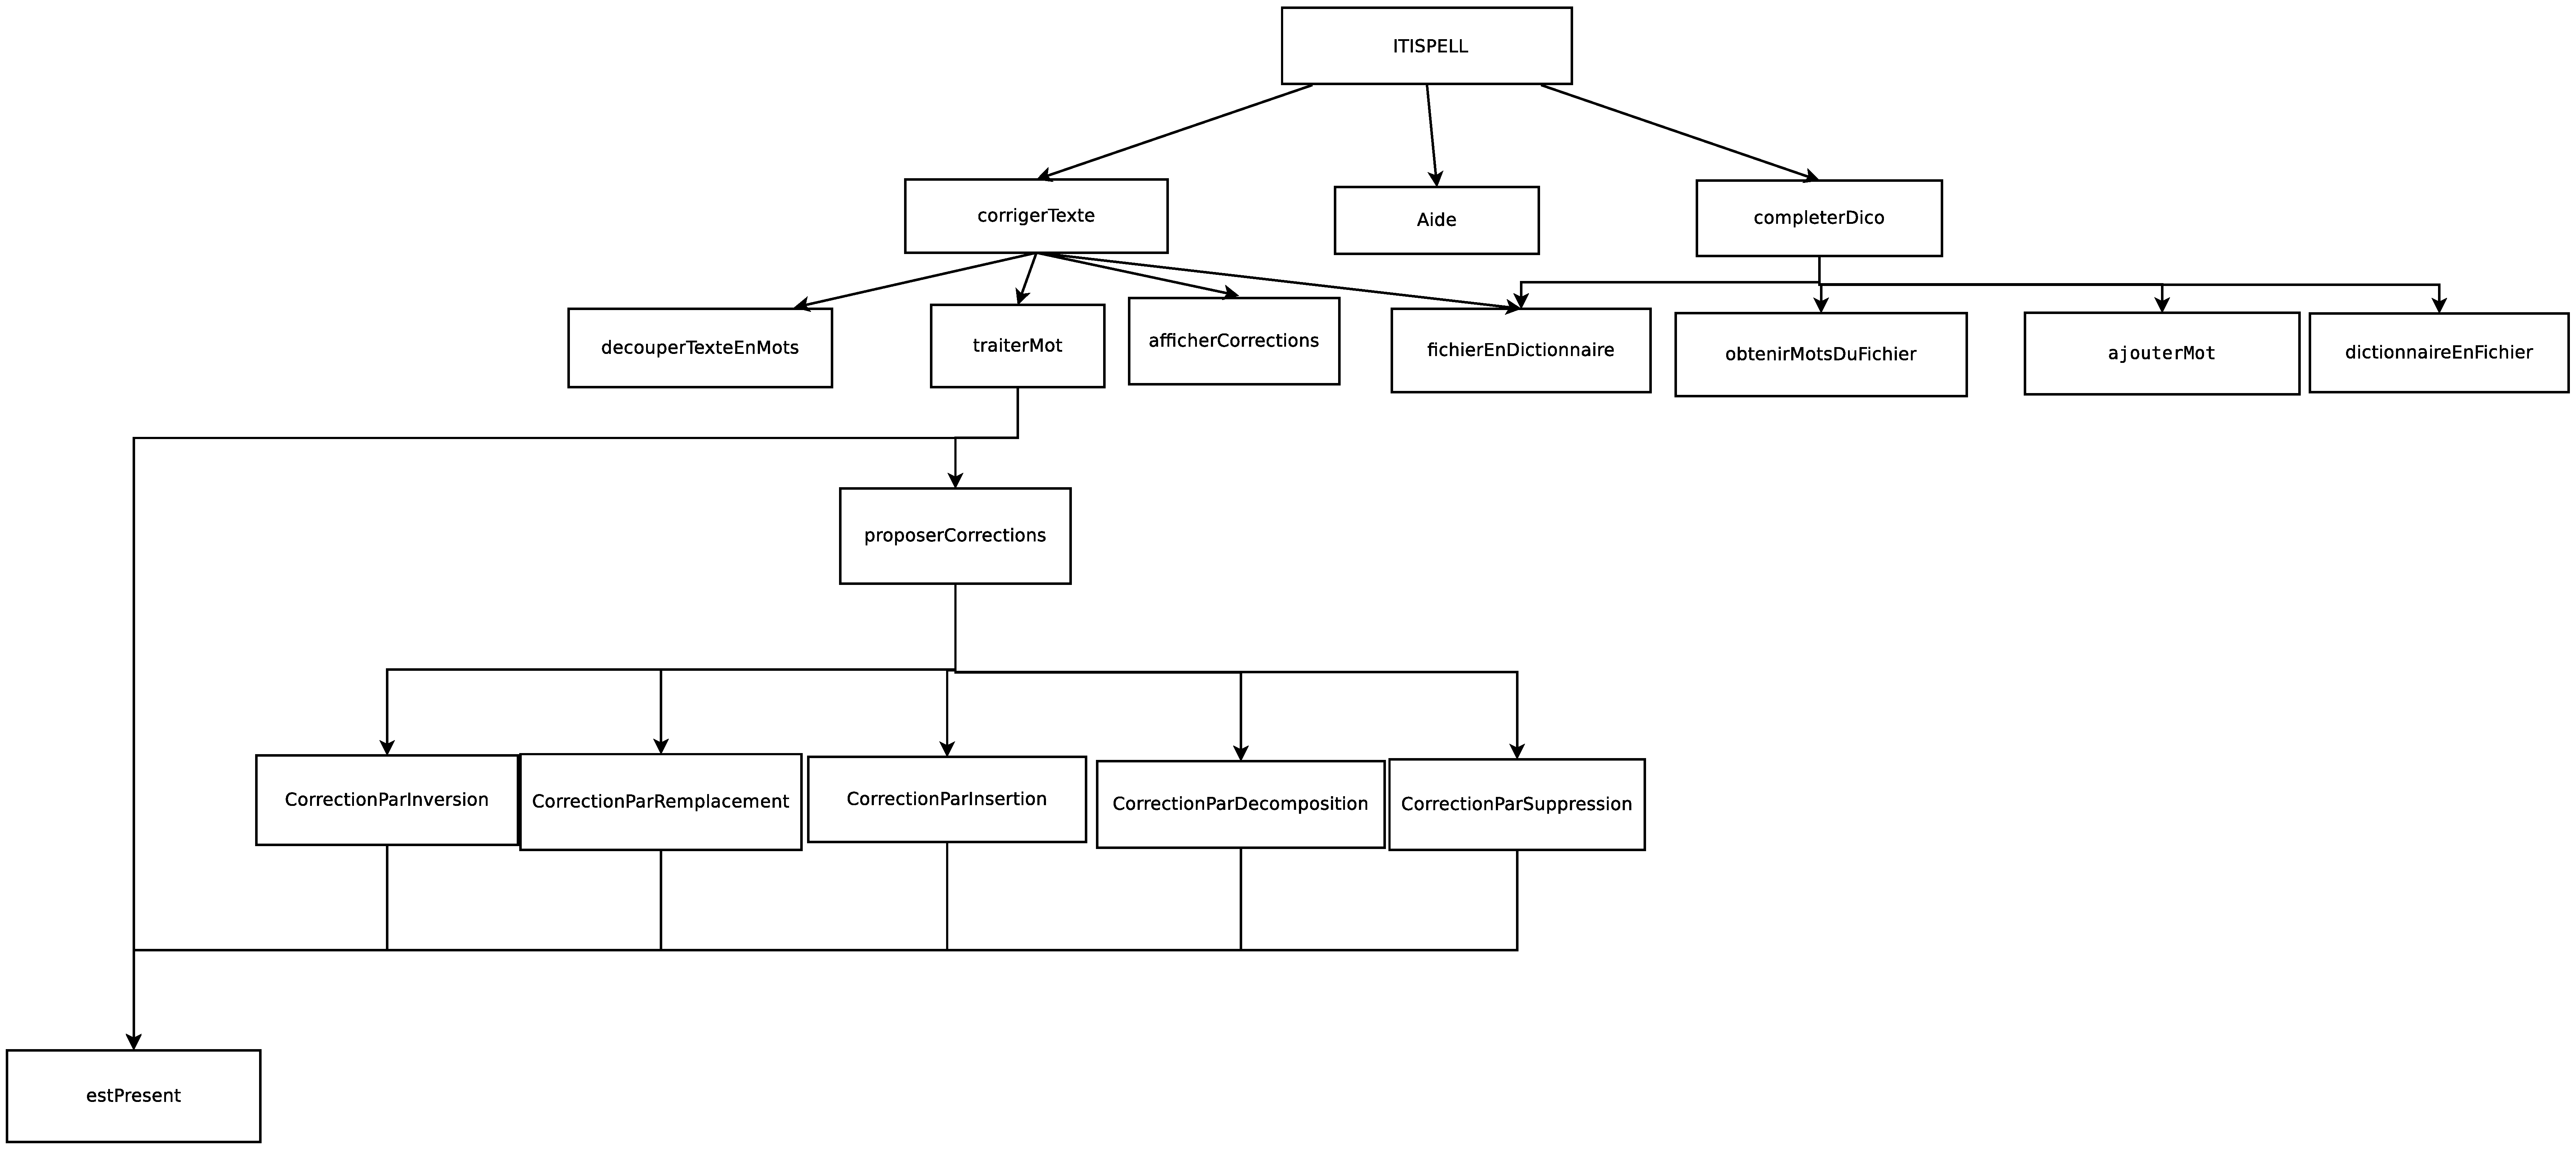
\includegraphics[width=\textwidth]{images/AD_globale.eps}
	\caption{Analyse descendante globale du projet}
	\label{fig:ADglobale}
\end{figure}
\begin{figure}[H]
	\centering 
	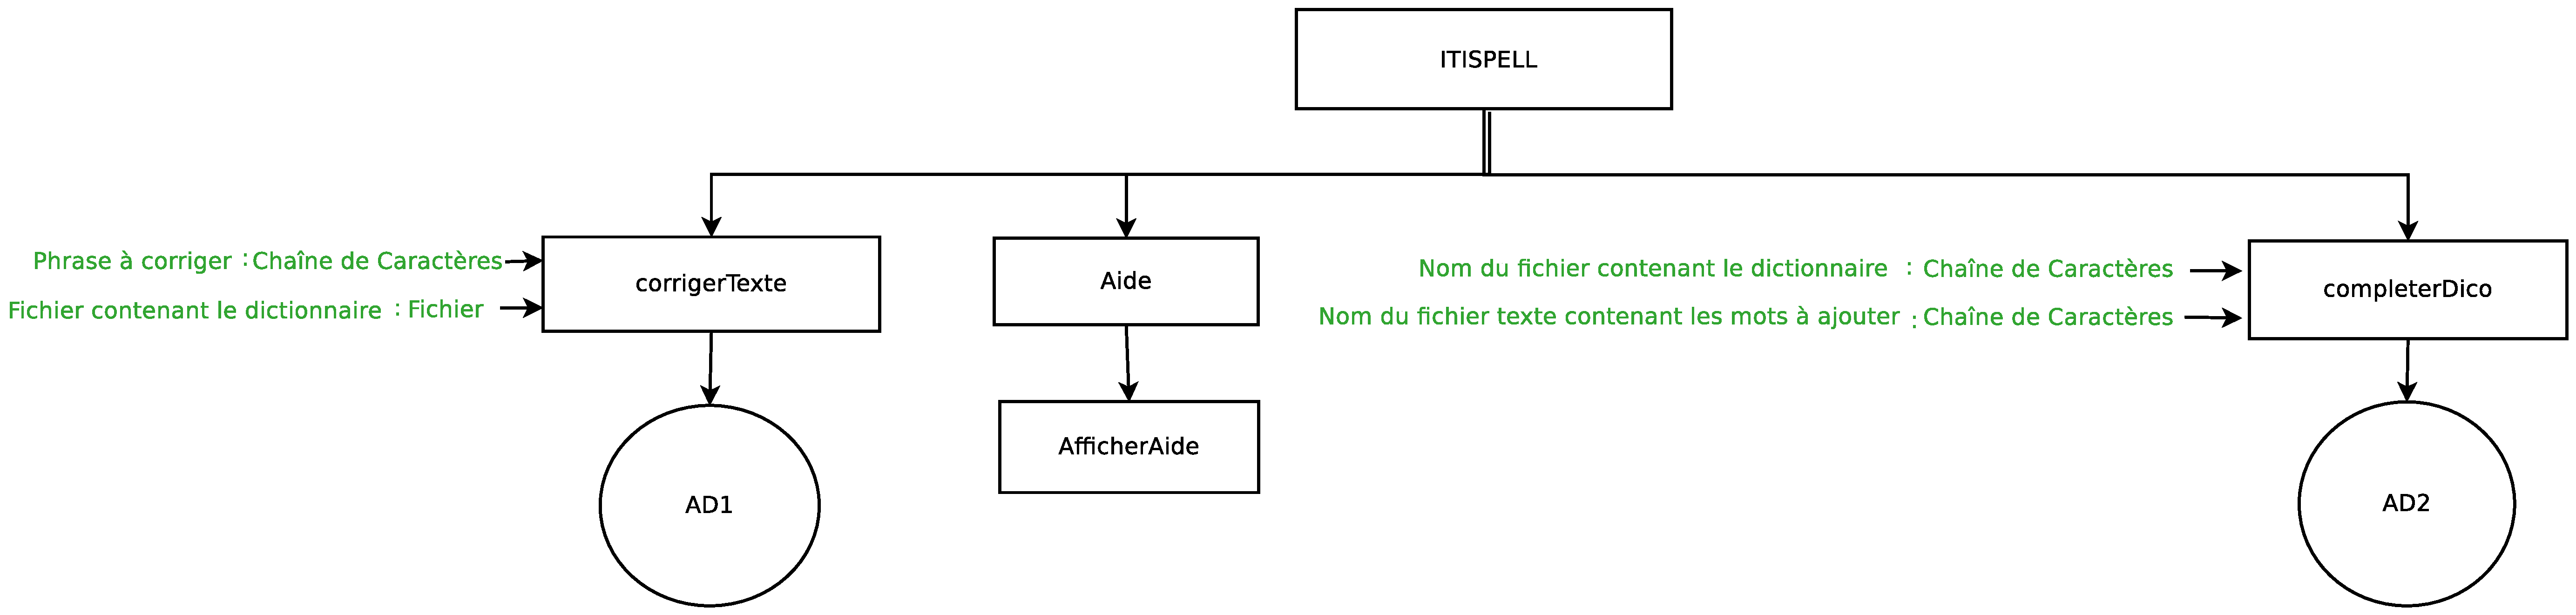
\includegraphics[width=\textwidth, angle=90, scale = 1.3]{images/AD0.eps}
	\caption{Analyse descendante simplifiée (AD0)}
	\label{fig:AD0}
\end{figure}
\begin{figure}[H]
	\centering 
	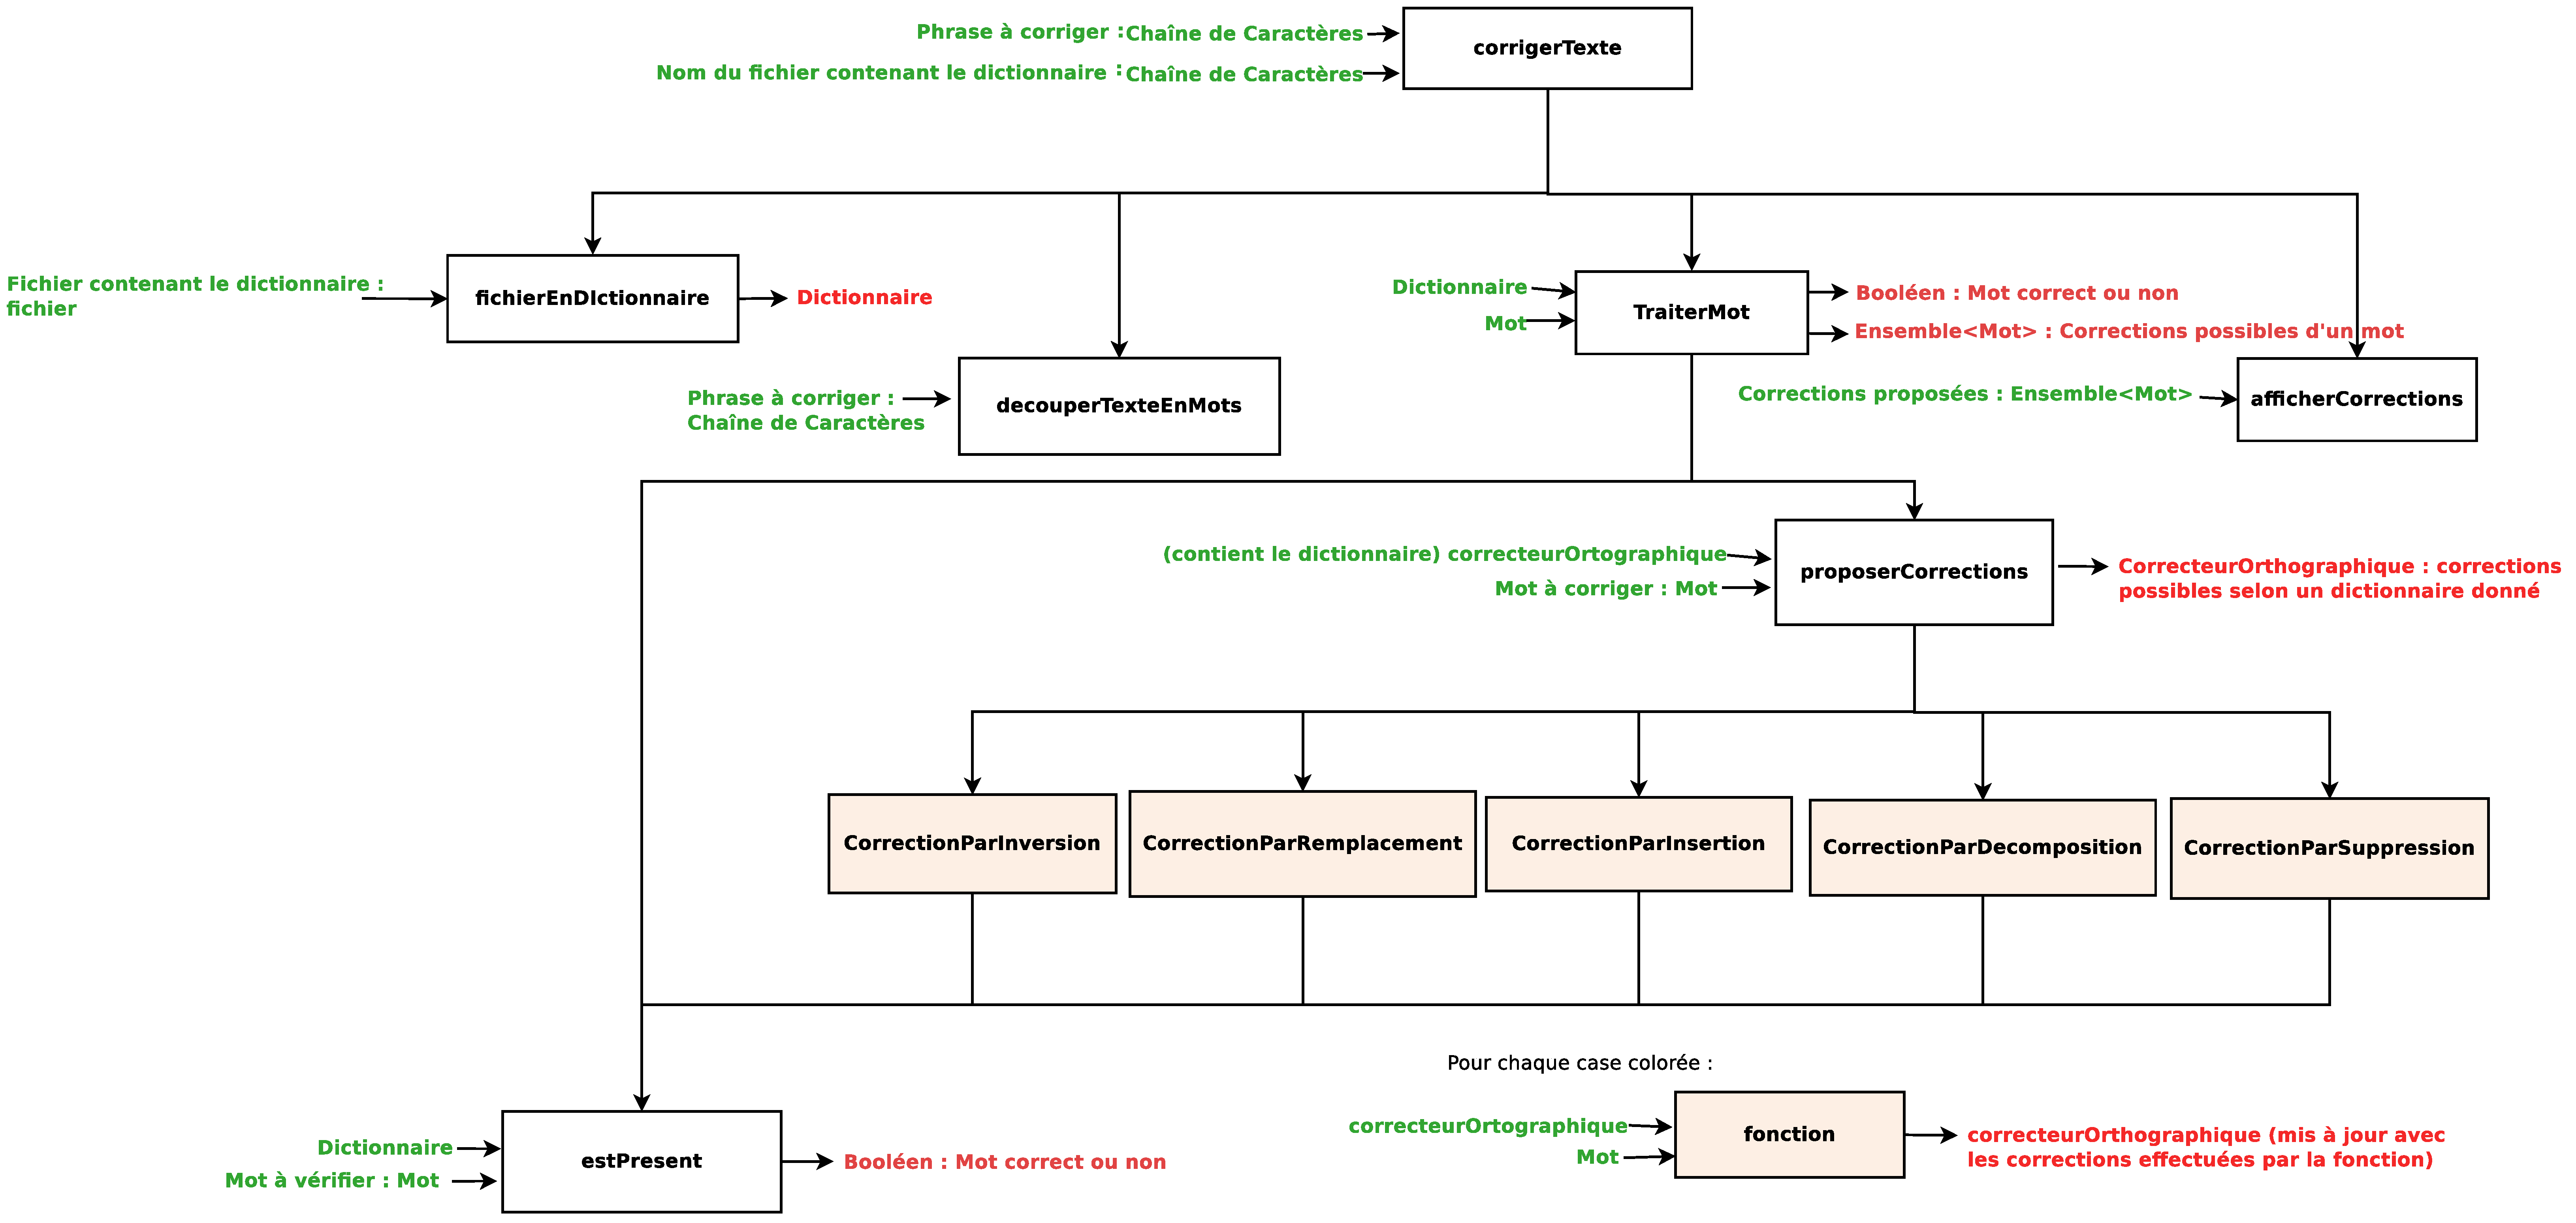
\includegraphics[width=\textwidth, angle=90, scale = 1.3]{images/AD1.eps}
	\caption{Analyse descendante de la partie correction (AD1)}
	\label{fig:AD1}
\end{figure}
\begin{figure}[H]
	\centering 
	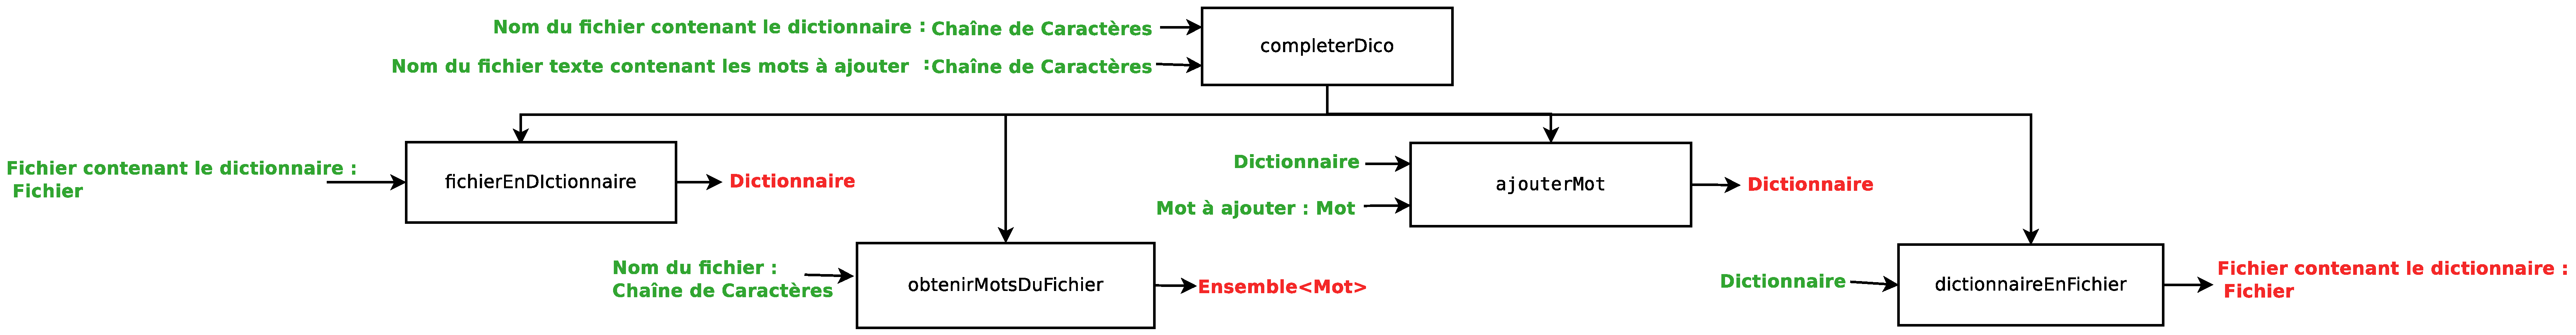
\includegraphics[width=\textwidth, angle=90, scale = 1.3]{images/AD2.eps}
	\caption{Analyse descendante de la partie complétion (AD2)}
	\label{fig:AD2}
\end{figure}
\newpage
\section{Conception préliminaire}
    \subsection{Signature des procédures et fonctions issues des TAD}
        %\documentclass[11pt,a4paper]{article}
%\usepackage{algorithmeUTF8}
%\usepackage{classeRapport}

%\begin{document}

\subsubsection{TAD Mot}
    \begin{algorithme}
        \signatureFonctionAvecPreconditions{creerMot}{CdC : \chaine}{Mot}{estUnMot(CdC)}
        \signatureFonction{longueur}{mot : Mot}{\naturel}
        \signatureFonction{estUnMot}{CdC : \chaine}{\booleen}
        \signatureFonctionAvecPreconditions{iemeCaractere}{mot : Mot, i : \naturelNonNul}{\caractere}{i $\leq$ longueur(mot)}
        \signatureFonctionAvecPreconditions{remplaceLettre}{mot : Mot, c : \caractere, i : \naturelNonNul}{Mot}{i $\leq$ longueur(mot)}
        \signatureFonctionAvecPreconditions{inverseLettres}{mot : Mot, i : \naturelNonNul}{Mot}{i $<$ longueur(mot)}
        \signatureFonctionAvecPreconditions{supprimeLettre}{mot : Mot, i : \naturelNonNul}{Mot}{longueur(mot) $\geq$ 2 et i $\leq$ longueur(mot)}
        \signatureFonctionAvecPreconditions{insereLettre}{mot : Mot, c : \caractere, i : \naturelNonNul}{Mot}{i $\leq$ longueur(mot)+1 et estUnCaractereValide(c)}
        \signatureFonctionAvecPreconditions{decomposeMot}{mot : Mot, i : \naturelNonNul}{Mot, Mot}{longueur(mot) $\geq$ 2 et i $\leq$ longueur(mot)-1}
        \signatureFonction{estUnCaractereValide}{c : \caractere}{\booleen}
\end{algorithme}

\subsubsection{TAD Dictionnaire}
    \begin{algorithme}
        \signatureFonction{creerDictionnaire}{}{Dictionnaire}
        \signatureFonction{estVide}{dico : Dictionnaire}{\booleen}
        \signatureProcedure{ajouteMot}{\paramEntreeSortie{dico : Dictionnaire}, \paramEntree{mot : Mot}}
        \signatureFonctionAvecPreconditions{estPresent}{dico : Dictionnaire, mot : Mot}{\booleen}{non estVide(dico)}
        \signatureProcedureAvecPreconditions{dictionnaireEnFichier}{\paramEntreeSortie{fdico : Fichier}, \paramEntree{dico : Dictionnaire}}{estOuvert(fdico)}
        \signatureProcedureAvecPreconditions{fichierEnDictionnaire}{\paramEntreeSortie{dico : Dictionnaire}, \paramEntree{fdico : Fichier}}{estOuvert(fdico)}
    \end{algorithme}

\subsubsection{TAD Correcteur Orthographique}
    \begin{algorithme}
        \signatureFonction{creerCorrecteur}{dico : Dictionnaire}{Correcteur Orthographique}
        \signatureProcedureAvecPreconditions{corrigeParInversion}{mot : Mot, corr : Correcteur Orthographique}{longueur(mot) $\geq$ 2}
        \signatureProcedure{corrigeParInsertion}{\paramEntreeSortie{corr : Correcteur Orthographique}, \paramEntree{mot : Mot}}
        \signatureProcedureAvecPreconditions{corrigeParDecomposition}{\paramEntreeSortie{corr : Correcteur Orthographique}, \paramEntree{mot : Mot}}{longueur(mot) $\geq$ 2}
        \signatureProcedureAvecPreconditions{corrigeParSuppression}{\paramEntreeSortie{corr : Correcteur Orthographique}, \paramEntree{mot : Mot}}{longueur(mot) $\geq$ 2}
        \signatureProcedureAvecPreconditions{corrigeParRemplacement}{\paramEntreeSortie{corr : Correcteur Orthographique}, \paramEntree{mot : Mot}}{longueur(mot) $\geq$ 2}
    \end{algorithme}

%\end{document}
    \subsection{Signature des procédures et fonctions issues de l'analyse}
        %\documentclass[11pt,a4paper]{article}
%\usepackage{algorithmeUTF8}
%\usepackage{classeRapport}

%\begin{document}

\subsubsection{AD0}
\begin{algorithme}
    \signatureProcedure{itispell}{}
    \signatureProcedure{corrigerPhrase}{phraseACorriger : \chaine, fdico : Fichier}
    \signatureProcedure{aide}{}
    \signatureProcedure{afficherAide}{}
    \signatureProcedure{completerDico}{fichierMots : Fichier, fdico : Fichier}
\end{algorithme}

\subsubsection{AD1}
\begin{algorithme}
    \signatureFonction{decouperTexteEnMots}{phraseACorriger : \chaine}{Ensemble <Mot>}
    \signatureFonction{traiterMot}{dico : Dictionnaire, mot : Mot}{\booleen, Ensemble <Mot>}
    \signatureProcedure{afficherCorrections}{\paramEntree{Ensemble <Mot>}}
    \signatureProcedure{proposerCorrections}{\paramEntreeSortie{corr : Correcteur Orthographique}, \paramEntree{motACorriger : Mot}}
\end{algorithme}

\subsubsection{AD2}
\begin{algorithme}
    \signatureFonction{completerDictionnaire}{fdico, fmots : Fichier}{Dictionnaire} %pas convaincue
    \signatureFonction{obtenirMotsDuFichier}{fichier : Fichier}{Ensemble <Mot>}
\end{algorithme}


%\end{document}
\newpage
\section{Conception détaillée}
    \subsection{Conception détaillée des fonctions issues des TAD}
    	%\documentclass[11pt,a4paper]{article}
%\usepackage{algorithmeUTF8}
%\usepackage{classeRapport}

%\begin{document}

\subsubsection{TAD Mot}
	\begin{algorithme}
		\begin{enregistrement}{Mot}
			\champEnregistrement{data}{\chaine}
			\champEnregistrement{longueur}{\naturel}
		\end{enregistrement}\\

		\fonctionAvecPreconditions{creerMot}%
		{CdC : \chaine}%
		{Mot}%
		{estUnMot(CdC)}%
		{mot : Mot}%
		{\affecter{mot.data}{CdC}
		\affecter{mot.longueur}{longueurChaine(CdC)}
		\retourner{mot}
		}\\
		
        \fonction{estUnMot}%
        {mot : Mot}%
        {\booleen}%
        {resultat : \booleen, i : \naturelNonNul}%
        {\affecter{resultat}{VRAI}%
        \affecter{i}{1}%
        \tantque%
        	{resultat et i $\leq$ longueur(mot)}%
        	{\affecter{i}{i+1}%
        	\affecter{resultat}{estUnCaractereValide(iemeCaractere(mot, i))}
        	}
        \retourner{resultat}
        }\\
		
        \fonctionAvecPreconditions{remplaceLettre}%
        {mot : Mot, c : \caractere, i : \naturelNonNul}%
		{Mot}%
        {i $\leq$ longueur(mot)}%
        {testMot : Mot}%
		{\affecter{testMot}{copieMot(mot)}%
		\instruction{modifieiemeCaractere(testMot, c, i)}%
		\retourner{testMot}}\\
        
        \fonctionAvecPreconditions{inverseLettres}%
        {mot : Mot, i : \naturelNonNul}%
		{Mot}%
        {i $<$ longueur(mot)}%
        {testMot : Mot, c1, c2 : \caractere}%
        {\affecter{testMot}{copieMot(mot)}%
		\affecter{c1}{obtenirIemeCaractere(testMot, i)}%
		\affecter{c2}{obtenirIemeCaractere(testMot, i $+$ 1)}%
		\instruction{echanger(c1, c2)}%
		\retourner{testMot}}\\
        
        \fonctionAvecPreconditions{supprimeLettre}%
        {mot : Mot, i : \naturelNonNul}%
		{Mot}%
        {longueur(mot) $\geq$ 2 et i $\leq$ longueur(mot)}%
        {data, dataTest : \chaine, j : \naturelNonNul, testMot : Mot}%
        {\affecter{data}{obtenirData(mot)}%
		\affecter{dataTest}{""}%
		\pour{j}{1}{longueur(mot)}{}%
			{\sialors{j $\neq$ i}%
				{\instruction{ajouteriemeCaractere(dataTest, data, j)}}
			}
		\affecter{testMot}{creerMot(dataTest)}%
		\retourner{testMot}}\\
        
        \fonctionAvecPreconditions{insereLettre}%
        {mot : Mot, c : \caractere, i : \naturelNonNul}%
		{Mot}%
        {i $\leq$ longueur(mot)+1 et estUnCaractereValide(c)}%
        {data, dataTest : \chaine, j : \naturelNonNul, testMot : Mot}%
        {\affecter{data}{obtenirData(mot)}%
		\affecter{dataTest}{""}%
		\pour{j}{1}{longueur(mot)}{}%
			{\sialors{j $=$ i}%
				{\instruction{ajouterCaractere(dataTest, c)}}%
			\instruction{ajouteriemeCaractere(dataTest, data, j)}
			}%
		\affecter{testMot}{creerMot(dataTest)}%
		\retourner{testMot}}\\
        
        \fonctionAvecPreconditions{decomposeMot}%
        {mot : Mot, i : \naturelNonNul}%
        {Mot, Mot}%
        {longueur(mot) $\geq$ 2 et i $\leq$ longueur(mot)-1}%
        {dataTest, dataTest1, dataTest2 : \chaine, j : \naturelNonNul, testMot1, testMot2 : Mot}%
        {\affecter{data}{obtenirData(mot)}%
		\affecter{dataTest1}{""}%
		\affecter{dataTest2}{""}%
		\pour{j}{1}{i $-$ 1}{}%
			{\instruction{ajouteriemeCaractere(dataTest1, data, j)}}%
		\pour{j}{i}{longueur(mot)}{}%
			{\instruction{ajouteriemeCaractere(dataTest2, data, j)}}%
		\affecter{testMot1}{creerMot(dataTest1)}%
		\affecter{testMot2}{creerMot(dataTest2)}%
		\retourner{testMot1, testMot2}}
	\end{algorithme}

\subsubsection{TAD Dictionnaire}
	\begin{algorithme}
		\begin{enregistrement}{Dictionnaire}
			\champEnregistrement{dico}{ArbreNaire}
		\end{enregistrement}\\
		
		\begin{enregistrement}{ArbreNaire}
			\champEnregistrement{e}{Element}
			\champEnregistrement{fils}{Liste Chainee <Dictionnaire>}
			\champEnregistrement{nbFils}{\naturel}
		\end{enregistrement}\\
		
		\begin{enregistrement}{Element}
			\champEnregistrement{caractere}{\caractere}
			\champEnregistrement{motExiste}{\booleen}
		\end{enregistrement}\\
		
		\fonction{dictionnaire}%
		{}%
		{Dictionnaire}%
		{}%
		{\retourner{arbreNaire()}}\\
		
		\fonction{estVide}%
		{dico : Dictionnaire}%
		{\booleen}%
		{}%
		{\retourner{obtenirCaractere(obtenirArbre(dico)) $=$ ""}}\\
		
		\fonctionAvecPreconditions{estPresent}%
		{dico : Dictionnaire, mot : Mot}%
		{\booleen}%
		{non estVide(dico)}
		{trouve, estPresent : \booleen, i, j : \naturel, l : Liste Chainee <ArbreNaire>, a : ArbreNaire}%
		{\affecter{estPresent}{FAUX}%
		\affecter{trouve}{VRAI}%
		\affecter{i}{1}%
		\affecter{a}{obtenirArbre(dico)}
		\tantque%
			{non trouve et j $\leq$ obtenirNbFils(a)}%
			{\sialorssinon%
				{obtenirIemeCaractere(mot, i) $=$ obtenirCaractere(obtenirElementLC)}
				{\affecter{trouver}{VRAI}}
				{\affecter{l}{obtenirListeSuivante(l)}
				\affecter{j}{j+1}}
			}%
		\sialors%
			{trouve}
			{\sialors%
				{(i $=$ longueur(mot)) et obtenirBooleen(a)}
				{\affecter{estPresent}{VRAI}}
			\affecter{i}{i+1}
			\affecter{a}{obtenirElementLC(l)}
			}
		}\\
		
		\procedure{ajouteMot}%
		{\paramEntreeSortie{dico : Dictionnaire}, \paramEntree{mot : Mot}}%
		{trouve, motAjoute : \booleen, i, j : \naturelNonNul, l : Liste Chainee <ArbreNaire>, temp : ArbreNaire}
		{\affecter{motAjoute}{FAUX}%
		\affecter{trouve}{VRAI}%
		\affecter{i}{1}%
		\affecter{a}{obtenirArbre(dico)}%
		\tantque%
			{non motAjoute et i $\leq$ longueur(mot)}%
			{\affecter{l}{obtenirFils(a)}%
			\affecter{j}{1}%
			\affecter{trouve}{FAUX}%
			\tantque%
				{non trouve et j $\leq$ obtenirNbFils(a)}%
				{\sialorssinon%
					{obtenirIemeCaractere(mot, i) $=$ obtenirCaractere(obtenirElementLC(l))}%
					{\affecter{trouve}{VRAI}}%
					{\affecter{l}{obtenirListeSuivante(l)}%
					\affecter{j}{j+1}}%
				}%
			\sialorssinon%
				{trouve}%
				{\sialors%
					{i $=$ longueur(mot)}%
					{\sialors%
						{non obtenirBooleen(a)}%
						{\instruction{fixerBooleen(a, VRAI)}}%
					\affecter{a}{obtenirElementLC(l)}%
					}%
				}%
				{\affecter{temp}{arbreNaire()}%
				\instruction{fixerCaractere(temp, obtenirIemeCaractere(mot, i))}%
				\sialorssinon%
					{i $=$ longueur(m)}%
					{\instruction{fixerBooleen(temp, VRAI)}%
					\affecter{motAjoute}{VRAI}}%
					{\instruction{fixerBooleen(temp, FAUX)}}%
				\instruction{fixerFils(a, temp)}%
				\instruction{fixerNbFils(a, obtenirNbFils(a) $+$ 1)}%
				}%
			\affecter{i}{i+1}%
			}
		}\\
		
		\procedureAvecPreconditions{dictionnaireEnFichier}%
		{\paramEntreeSortie{fdico : Fichier}, \paramEntree{dico : Dictionnaire}}%
		{estOuvert(fdico)}%
		{temp : Liste Chainee <ArbreNaire <Element>>, a : ArbreNaire <Element>, i : \naturel}%
		{\affecter{a}{obtenirArbre(dico)}%
		\sialors%
			{non estVide(a)}%
			{\instruction{ecrireCaractere(fdico, obtenirCaractere(a))}%
			\instruction{ecrireCaractere(fdico, obtenirBooleen(a))}%
			\instruction{ecrireCaractere(fdico, nbFils(a))}%
			\affecter{temp}{obtenirFils(a)}%
			\pour{i}{1}{obtenirNbFils(a)}{}%
				{\instruction{dictionnaireEnFichier(fdico, obtenirElement(temp))}%
				\affecter{temp}{obtenirListeSuivante(temp)}
				}
			}
		}\\
		
        \procedureAvecPreconditions{fichierEnDictionnaire}%
        {\paramEntreeSortie{dico : Dictionnaire}, \paramEntree{fdico : Fichier}}%
        {estOuvert(fdico)}%
        {temp, a : AbreNaire <Element>, i : \naturelNonNul, nbFils : \naturel, c : \caractere, bool : \booleen}%
        {\affecter{a}{obtenirArbre(d)}%
        \sialors%
        	{non finFichier(fdico)}%
        	{\affecter{fdico, c}{lireCaractere(fdico)}%
        	\instruction{fixerCaractere(a, c)}%
        	\affecter{fdico, bool}{lireCaractere(fdico)}%
        	\instruction{fixerBooleen(a, bool)}%
        	\affecter{fdico, nbFils}{lireCaractere(fdico)}%
        	\instruction{fixerNbFils(a, nbFils)}%
        	\affecter{temp}{arbreNaire()}%
        	\pour{i}{1}{nbFils}{}%
        		{\instruction{fichierEnDictionnaire(temp, fdico)}%
        		\instruction{fixerFils(a, temp)}%
        		}%
        	}
        }
	\end{algorithme}

\subsubsection{TAD Correcteur Orthographique}
	\begin{algorithme}
		\begin{enregistrement}{Correcteur Orthographique}
			\champEnregistrement{dictionnaire}{Dictionnaire}
			\champEnregistrement{corrections}{Ensemble <Mot>}
		\end{enregistrement}\\
		
		\fonction{creerCorrecteur}%
		{dico : Dictionnaire}%
		{Correcteur Orthographique}%
		{corr : Correcteur Orthographique}%
		{\affecter{corr.dictionnaire}{dico}%
		\affecter{corr.corrections}{ensemble()}%
		\retourner{corr}}\\
		
		\procedureAvecPreconditions{corrigeParInversion}%
		{\paramEntreeSortie{corr : Correcteur Orthographique}, \paramEntree{mot : Mot}}%
		{longueur(mot) $\geq$ 2}%
		{i : \naturelNonNul, testMot : Mot}%
		{\pour{i}{1}{longueur(mot) $-$ 1}{}%
			{\affecter{testMot}{inversionLettres(mot, i)}%
			\sialors%
				{estPresentDansDictionnaire(testMot, corr)}%
				{\instruction{ajouteCorrection(corr, testMot)}}%
			}%
		}\\
		
		\procedure{corrigeParInsertion}%
		{\paramEntreeSortie{corr : Correcteur Orthographique}, \paramEntree{mot : Mot}}%
		{i, j : \naturelNonNul, testMot: Mot}
		{\pour{i}{1}{longueur(mot) $+$ 1}{}{%
			\pour{j}{ord("a")}{ord("a")+26}{}{%
				\affecter{testMot}{inversionLettres(mot, i)}%
				\sialors%
					{estPresentDansDictionnaire(testMot, corr)}%
					{\instruction{ajouteCorrection(corr, testMot)}}%
				}
			}
		}\\
		
        \procedureAvecPreconditions{corrigeParDecomposition}%
        {\paramEntreeSortie{corr : Correcteur Orthographique}, \paramEntree{mot : Mot}}%
        {longueur(mot) $\geq$ 2}%
		{i : \naturelNonNul, testMot1, testMot2 : Mot}%
		{\pour{i}{1}{longueur(mot) $-$ 1}{}{%
			\affecter{testMot1, testMot2}{decomposerMot(mot, i)}
			\sialors%
				{estPresentDansDictionnaire(testMot1, corr)}%
				{\instruction{ajouteCorrection(corr, testMot1)}}%
			\sialors%
				{estPresentDansDictionnaire(testMot1, corr)}%
				{\instruction{ajouteCorrection(corr, testMot1)}}%
			}
		}\\
                
        \procedureAvecPreconditions{corrigeParSuppression}%
        {\paramEntreeSortie{corr : Correcteur Orthographique}, \paramEntree{mot : Mot}}%
        {longueur(mot) $\geq$ 2}%
		{i : \naturelNonNul, testMot: Mot}%
		{\pour{i}{1}{longueur(mot)}{}{%
			\affecter{testMot}{supprimeLettre(mot, i)}
			\sialors%
				{estPresentDansDictionnaire(testMot, corr)}%
				{\instruction{ajouteCorrection(corr, testMot)}}%
			}
		}\\
        
        \procedureAvecPreconditions{corrigeParRemplacement}%
        {\paramEntreeSortie{corr : Correcteur Orthographique}, \paramEntree{mot : Mot}}%
        {longueur(mot) $\geq$ 2}%
        {i, j : \naturelNonNul, testMot : Mot}
        {\pour{i}{1}{longueur(mot)}{}{%
			\pour{j}{ord("a")}{ord("a") $+$ 26}{}{%
				\affecter{testMot}{remplaceLettre(mot, i)}%
				\sialors%
					{estPresentDansDictionnaire(testMot, corr)}%
					{\instruction{ajouteCorrection(corr, testMot)}}%
				}
			}
		}\\
	\end{algorithme}

%\end{document}
    \subsection{Conception détaillée des fonctions issues de l'analyse descendante}
        \subsubsection{AD0}
	\begin{algorithme}
        \procedure{corrigerPhrase}%
        {\paramEntree{phraseACorriger : \chaine, fdico : Fichier}}%
        {dico : Dictionnaire, mot : Mot, motsACorriger, corrections : Ensemble <Mot>, i : \naturelNonNul}%
        {\affecter{dico}{fichierEnDictionnaire(fdico)}
        \affecter{motsACorriger}{decouperTexteEnMots(phraseACorriger)}
        \pourChaque{mot}{motsACorriger}%
        	{\sialorssinon{estPresent(dico, mot)}%
    	        {\ecrire{"*"}}%
        	    {\affecter{corrections}{traiterMot(dico, mot)}
            	\instruction{afficherCorrections(mot, corrections)}
            	}
            }%
        }\\
    \end{algorithme}

\subsubsection{AD1}
    \begin{algorithme}
        \fonction{decouperTexteEnMots}%
        {phraseACorriger : \chaine}%
        {Ensemble <Mot>}%
        {ens : Ensemble <Mot>, i : \naturelNonNul, temp : \chaine}%
        {\affecter{temp}{""}
        \pour{i}{1}{longueur(phraseACorriger)}{}%
            {\tantque{iemeCaractere(phraseACorriger, i) $\neq$ " "}%
                {\affecter{temp}{temp $+$ iemeCaractere(phraseACorriger, i)}}
            \instruction{ajouter(ens, creerMot(temp))}
            \affecter{temp}{""}
            }
        \retourner{ens}
        }\\
        
        \fonction{traiterMot}%
        {dico : Dictionnaire, mot : Mot}%
        {\booleen, Ensemble <Mot>}%
        {corr : Correcteur}%
        {\sialorssinon{estPresent(dico, mot)}
            {\retourner{VRAI, ensemble()}}
            {\affecter{corr}{creerCorrecteur(dico)}%
            \instruction{proposerCorrections(corr, mot)}%
            \retourner{FAUX, obtenirCorrections(corr)}}
        }\\

        \procedure{proposerCorrections}%
        {\paramEntreeSortie{corr : Correcteur Orthographique}, \paramEntree{motACorriger : Mot}}%
        {}%
        {\instruction{corrigeParInvertion(corr, motACorriger)}
        \instruction{corrigeParInsertion(corr, motACorriger)}
        \instruction{corrigeParDecomposition(corr, motACorriger)}
        \instruction{corrigeParSuppression(corr, motACorriger)}
        \instruction{corrigeParRemplacement(corr, motACorriger)}}
    \end{algorithme}

\subsubsection{AD2}
\begin{algorithme}    
    \fonction{obtenirMotsDuFichier}%
    {fichier : Fichier}%
    {Ensemble <Mot>}%
    {ensembleMots : Ensemble <Mot>, mot : Mot, CdC : \chaine}%
    {\tantque{non finFichier(fichier)}
        {\affecter{fichier, CdC}{lireChaine(fichier)}
        \affecter{CdC}{minuscule(CdC)}
        \affecter{mot}{creerMot(CdC)}
        \instruction{ajouter(ensembleMots, mot)}
        }
    \retourner{ensembleMots}
    }
\end{algorithme}
\newpage
\section{Code C et tests unitaires}
        En essayant de développer en C les fonctions détaillées précédemment, nous avons rencontré diverses problèmes et avons du faire quelques adaptations.

    En effet, pour le correcteur orthographique par exemple, nous avons changé notre idée de stocker toutes les corrections dans un ensemble de mots pour utiliser plutôt une liste chaînée à la place.
    Ainsi, l'implémentation de la liste chaînée que nous devions déjà faire pour le dictionnaire nous a finalement aussi servi dans le correcteur orthographique.

    De plus, nous avons également adapté la fonction completerDico en C. Dans l'analyse descendante, celle-ci devait utiliser différentes fonctions (notamment obtenirMotsDuFichier, mais nous avons choisi lors de l'implémentation de les coder ensemble toutes les deux.
    \subsection{Code C}
       \definecolor{darkWhite}{rgb}{0.94,0.94,0.94}
 
\lstset{
  backgroundcolor=\color{darkWhite},
  basicstyle=\footnotesize,
  breakatwhitespace=false,
  breaklines=true,
  captionpos=b,
  commentstyle=\color{red},
  deletekeywords={...},
  escapeinside={\%*}{*)},
  extendedchars=true,
  framexleftmargin=16pt,
  framextopmargin=3pt,
  framexbottommargin=6pt,
  frame=tb,
  keepspaces=true,
  keywordstyle=\color{blue},
  language=C,
  literate=
  {²}{{\textsuperscript{2}}}1
  {⁴}{{\textsuperscript{4}}}1
  {⁶}{{\textsuperscript{6}}}1
  {⁸}{{\textsuperscript{8}}}1
  {€}{{\euro{}}}1
  {é}{{\'e}}1
  {è}{{\`{e}}}1
  {ê}{{\^{e}}}1
  {ë}{{\¨{e}}}1
  {É}{{\'{E}}}1
  {Ê}{{\^{E}}}1
  {û}{{\^{u}}}1
  {ù}{{\`{u}}}1
  {â}{{\^{a}}}1
  {à}{{\`{a}}}1
  {á}{{\'{a}}}1
  {ã}{{\~{a}}}1
  {Á}{{\'{A}}}1
  {Â}{{\^{A}}}1
  {Ã}{{\~{A}}}1
  {ç}{{\c{c}}}1
  {Ç}{{\c{C}}}1
  {õ}{{\~{o}}}1
  {ó}{{\'{o}}}1
  {ô}{{\^{o}}}1
  {Õ}{{\~{O}}}1
  {Ó}{{\'{O}}}1
  {Ô}{{\^{O}}}1
  {î}{{\^{i}}}1
  {Î}{{\^{I}}}1
  {í}{{\'{i}}}1
  {Í}{{\~{Í}}}1,
  morekeywords={*,...},
  numbers=left,
  numbersep=10pt,
  numberstyle=\tiny\color{black},
  rulecolor=\color{black},
  showspaces=false,
  showstringspaces=false,
  showtabs=false,
  stepnumber=1,
  stringstyle=\color{gray},
  tabsize=4,
  title=\lstname,
}

\subsubsection{Fichier TADMot.c}
	\lstinputlisting{../programme/src/TAD_Mot.c}
\subsubsection{Fichier TADDictionnaire.c}
	\lstinputlisting{../programme/src/TAD_Dictionnaire.c}
\subsubsection{Fichier TADCorrecteur.c}
	\lstinputlisting{../programme/src/TAD_Correcteur.c}

\subsubsection{Implémentation des fonctions issues de l'analyse descendante}
	\lstinputlisting{../programme/src/main.c}
	\lstinputlisting{../programme/src/aide.c}
	\lstinputlisting{../programme/src/completerDico.c}
	\lstinputlisting{../programme/src/AD1.c}
    \subsection{Tests unitaires}
        \lstinputlisting{../programme/src/test.c}
\newpage
\section{Conclusion}
    \subsection{Conclusions par membres}
        \subsubsection{Victor Léger (chef de projet)}
            	Pour conclure, j’ai, grâce à ce projet, vu les différents aspects d’un vrai travail de groupe en informatique, car les derniers en date étaient ceux du projet informatique en STPI, mais il n’était pas aussi structuré que celui-ci et j’avais aussi fait un TIPNE au dernier semestre, mais j’étais tout seul.
Étant en équipe, nous nous sommes réparti les tâches et entraidé, ce qui me manquait dans mes autres projets.


	Au niveau informatique, le projet du correcteur orthographique m’a permis de me familiariser avec le langage de programmation C, car je n’en avais jamais fait avant et c’est mon premier projet en C. Ce qui m’a posé le plus de problème avec ce langage, ce sont bien évidemment les pointeurs et aussi de gérer l’espace mémoire lié à ses pointeurs. Nous avons eu beaucoup de « segmentation fault » durant le projet et c’était pour moi les erreurs les plus dures à comprendre.


	En tant que chef de projet, j’ai enfin pu comprendre l’utilisation de Gitlab, je pense qu’il y a encore beaucoup de commandes que je ne connais pas, mais j’ai déjà acquit les bases. Mon groupe était agréable et tout le monde accomplissait ses tâches dans le temps imparti. Nous avons fait régulièrement des réunions, au moins une fois par semaine, pour avoir un suivi de l’évolution du projet et chacun était présent. J’ai donc apprécié travailler avec les autres membres de ce groupe.
        \subsubsection{Cièle Gillet}
            	Ce projet d'algorithmique a été pour moi une toute nouvelle expérience. Etant intégrée à l'INSA, je n'avais auparavant jamais fait de projet en informatique (n'en ayant fait en CPGE qu'un seul en mécanique), ni de projet avec un groupe de 4 membres.
	
	Tout d'abord, le projet de correcteur orthographique m'a permis de mettre en application les cours d'algorithmique avancée et de programmation en C dans leur globalité, puisque nous devions réfléchir à la conception du correcteur en suivant les étapes du cycle en V. Cela a été très instructif pour moi, car je n'avais justement jamais appris à suivre ces étapes et je me suis donc rendu compte qu'il était primmordial d'avoir d'abord une idée claire de la structure du code avant de passer au développement ; en particulier lorsqu'il y a autant de fonctions et procédures que dans ce projet.
	
	J'ai également appris à utiliser de nouveaux outils tels que GIT et \LaTeX, ainsi que Doxygen pour la documentation et Valgrind qui nous a été d'une grande aide pour détecter les erreurs de notre code. Cependant, je pense qu'il m'a été difficile d'être efficace au commencement du projet justement à cause de ces différents outils que j'ai mis du temps à maîtriser (ne serait-ce que GIT pour envoyer mes documents aux autres membres du groupe).
	
	Ces deux derniers points (la conception générale du correcteur et la prise en main des nouveaux outils) m'ont donc pris beaucoup de temps. De plus, à cause d'un retard accumulé au cours des séances, nous avons dû consacrer une grande partie de nos vacances sur le projet, ce que je trouve déplorable surtout si l'on prend en compte les contraintes de toutes les autres matières de la ITI3.
	
	Finalement, j'ai trouvé que ce projet était très intéressant d'un point de vue pédagogique mais je regrette de ne pas avoir eu assez de temps pour le finaliser.
        \subsubsection{Rachida Imandou}
            	C'est la première fois que j'avais à réaliser un projet en C, ce projet m'a permis de mettre en pratique les cours théoriques sur le C, j'ai donc pu en comprendre le fonctionnement et découvrir les avantages et inconvénients de son utilisation : la gestion de la mémoire, les pointeurs, la compilation … et aussi j’ai familiarisé avec l’outil git et latex.


	Ce projet était une bonne occasion d'expérimenter le travail en équipe avec un cahier de charges, cette méthode m’a permis d’améliorer mes capacités d’adaptation avec différentes contraintes. 
        \subsubsection{Marilou Pascal}
            Lors de ce projet, j'ai pu gagner de l'expérience dans différents domaines, et pour cela je l'ai trouvé très intéressant. Le fait de devoir créer de A à Z un projet de cette ampleur représentait un vrai défi pour nous, et j'ai personnellement beaucoup apprécié la phase de conception préliminaire et d'analyse descendante où nous avons été amené à réfléchir par nous même. La spécification des TADs que nous allions utiliser était notamment très intéressante car elle a necessité de vraiment poser le problème et prendre du recul sur le projet.

Le deuxième point sur lequel j'ai pu progresser est la connaissance du langage C. Je n'avais jamais eu l'occasion de coder en C avant, et j'ai pu m'y initier à travers ce projet, ce que je trouve enrichissant pour le futur, étant donné le caractère non permissif du C et la rigueur qu'il exige.

Enfin je trouve que nous avons vraiment pu mesurer ce que signifiait le travail de groupe en informatique. J'avais déjà eu l'occasion de mener un projet à plusieurs en STPI en I3 puis en I4.2 (l'accent avait d'ailleurs été mis sur l'aspect collaboratif pour ce deuxième projet), et pouvoir le refaire au sein du departement ITI est réellement profitable. Nous avons pu constater la rigueur que cela exige dans la conception et dans le développement, et cela nous a permis de nous entraider afin de compenser les faiblesses de chacun.

Pour conclure je dirais que j'ai été contente de réaliser ce projet, le seul problème étant la charge de travail que j'ai trouvé trop conséquente par rapport au cursus ITI3, ce qui ne nous as pas permis de finaliser le programme. 


    \subsection{Conclusion générale}
        En conclusion, nous pouvons dire que ce projet nous aura permis de nous améliorer sur de nombreux points.

\bigskip

Tout d'abord, il nous a permis de nous familiariser avec le C et ses difficultés. En effet, ce langage n'étant pas permissif du tout, nous avons dû réfléchir avec beaucoup de rigueur à chaque aspect du programme, notamment la gestion des pointeurs. Cela a été un des éléments les plus compliqués à aborder et celui qui nous a posé le plus de problèmes au debuggage. Nous avons également découvert les joies de cette étape de debug, qui peut se révéler conséquente pour les programmes de cette envergure.

\bigskip

Autre apport de ce projet, nous avons pu appliquer concrètement des notions d'algorithmiques vues en cours, comme par exemple les arbres ou même les types abstraits de données, que nous n'avions jamais eu l'occasion de créer nous-même. Il était intéressant pour nous d'essayer de mettre en application ces notions de manière pertinente dans l'optique d’optimiser notre programme.

\bigskip

Ensuite, le travail de groupe nous a forcés à adopter une certaine rigueur dans notre approche du développement. Nous avons dû nous répartir les différentes tâches en fonction du niveau de compétence de chaque personne et de sa compréhension du sujet. Le fait de travailler à plusieurs nous a obligés à utiliser GitLab pour orchestrer au mieux le travail de groupe. Concernant l’utilisation de GitLab, cela n’a pas facile au début, mais chacun a réussi à comprendre le logiciel pour l’utiliser au mieux.

\bigskip

Pour conclure, à cause de la charge de travail et la difficulté du projet pour des débutants en C comme nous, nous n’avons pas mené à terme ce premier projet en C.

\bigskip

Nous avons aimé travailler sur ce projet même si malheureusement, nous n’avons pu le finir.
\end{document}